\documentclass[logo,reportComp]{thesis}
\usepackage{mypackage}

\title{机器学习与数据挖掘课堂作业}
\subtitle{决策树}
\school{数据科学与计算机学院}
\author{陈鸿峥}
\classname{17大数据与人工智能}
\stunum{17341015}
\headercontext{机器学习与数据挖掘课堂作业}

\begin{document}

\maketitle

\begin{question}
\normalfont Can decision trees solve non-linear classification problems? Why?
\end{question}
% https://discuss.analyticsvidhya.com/t/how-decision-tree-performs-non-linear-classification/6001
\begin{answer}
可以的,决策树通过不断划分属性值,从而可以解决非线性分类问题,只是决策树只能将特征空间\textbf{沿轴向}进行划分,如下面的例子所示。
\begin{figure}[H]
\centering
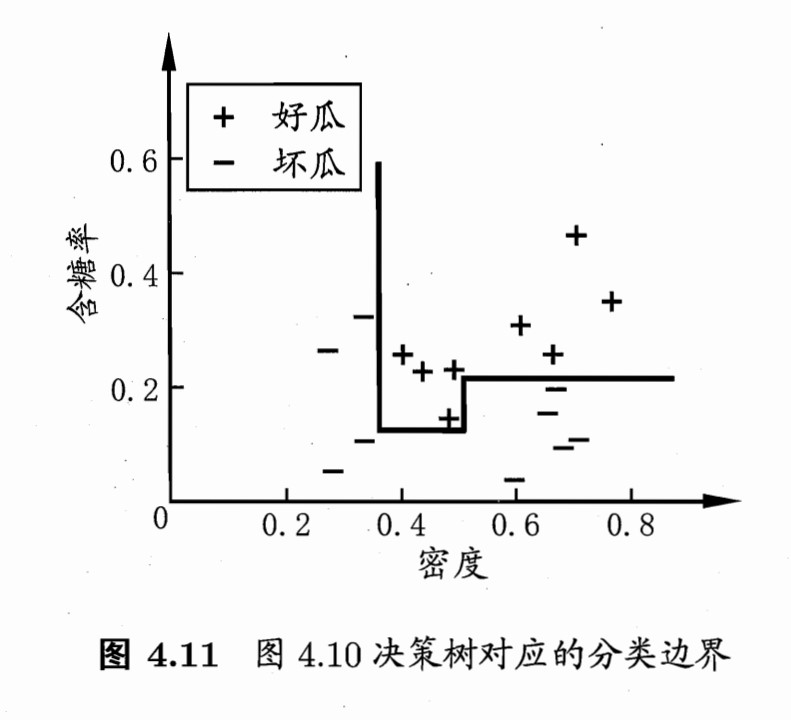
\includegraphics[width=0.6\linewidth]{fig/dt.jpg}
\end{figure}
\end{answer}

\end{document}